\documentclass[a4paper,12pt]{ctexart}
\usepackage{amsmath}
\usepackage{amsfonts}
\usepackage{float}
\usepackage{enumerate}
\usepackage{svg}
\usepackage{graphicx}
\usepackage{booktabs}
\usepackage[hidelinks]{hyperref}
\usepackage{multirow}
\usepackage{svg}
\setcounter{secnumdepth}{0}
\title{企业风险管理第一次作业}
\author{董晨阳 2201211201\thanks{\href{mailto:dongcy2018@econ.pku.edu.cn}{dongcy2018@econ.pku.edu.cn}}}
\date{\today}
\begin{document}
\maketitle
% \tableofcontents
% \listoffigures
% \clearpage
\section{SCA}
安全检查表如下表所示
\begin{table}[H]
    \caption{安全检查表}
    \centering
    \begin{tabular}{ccc}
        \toprule
        潜在安全问题        & 是否存在 & 备注                \\
        \midrule
        路线是否有足够的安全措施  &      & 护栏、标识危险地形等        \\
        应对突发事件的应急措施   &      & 应急响应系统与应急知识普及     \\
        选手是否健康        &      & 赛前身体检查和体能测试       \\
        选手是否合格        &      & 是否经过足够的准备和训练      \\
        是否存在恶劣的环境气候因素 &      & 建立相应的预警机制和应急响应计划  \\
        是否能监控赛事信息     &      & 利用传感器等确保预防安全事故发生  \\
        是否存在食品安全问题    &      & 赛事提供食物和水是否符合认证标准  \\
        是否存在网络安全漏洞    &      & 加强网络安全管理          \\
        选手装备是否专业      &      & 检查参赛选手的装备确保符合安全要求 \\
        是否影响交通        &      & 确保赛事与交通安全没有冲突     \\
        \bottomrule
    \end{tabular}
\end{table}
\section{JHA}
工作危害分析如下表所示
\begin{table}[H]
    \caption{工作危害分析}
    \centering
    \begin{tabular}{cccc}
        \toprule
        工作步骤                   & 危险源       & 主要后果       & 控制建议     \\
        \midrule
                               & 地形比较复杂、危险 & 受伤、摔落山崖    & 加装护栏     \\
                               & 选手身体素质不足  & 选手体力不支     & 体检       \\
                               & 选手装备不够    & 选手无法应对突发状况 & 提供部分装备   \\
                               & 疫情封控      & 选手无法到场     & 及时更改日程   \\
        \multirow{-5}{*}{赛前准备} & 选手间爆发疫情   & 被封控、感染     & 及时更改日程   \\
        \midrule
        & 选手突发不适    & 选手受伤       & 增加医护人员   \\
                               & 气候转劣      & 选手冻伤       & 及时更改日程   \\
                               & 通信措施坏掉    & 无法跟踪选手信息   & 准备更多传感器  \\
        \multirow{-4}{*}{赛中}   & 选手迷路      & 选手失联       & 路牌、志愿者指引 \\
        \midrule
        赛后                     & 废弃装备、水瓶遗落 & 环境污染       & 及时清理   \\

        \bottomrule
    \end{tabular}
\end{table}
\section{CCA}
原因-后果分析如下图所示
\begin{figure}[H]
    \caption{原因-后果分析}
    \centering
    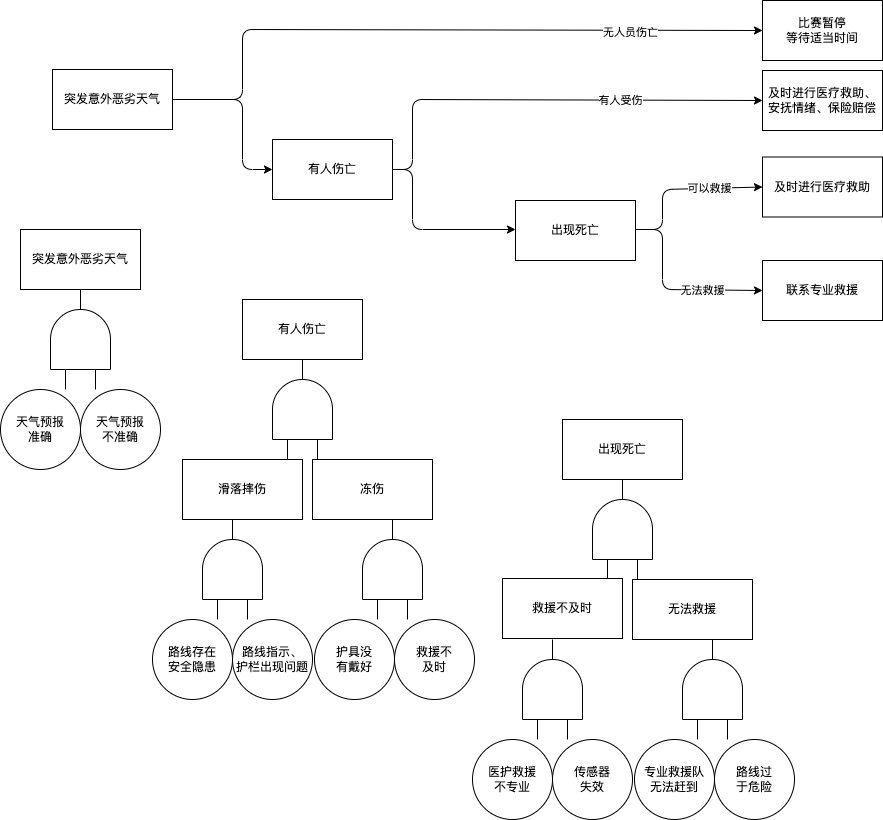
\includegraphics[width=\linewidth]{cca.drawio.png}
\end{figure}

\end{document}
